\documentclass[oneside, draft]{epstfg}

\usepackage{lipsum}
\usepackage[numbers]{natbib}
\usepackage{fancysprefs}

\usepackage{tikz}

\usetikzlibrary{arrows}
\usetikzlibrary{patterns}
\usetikzlibrary{intersections}
\usetikzlibrary{calc}
\usetikzlibrary{fadings}

\tikzset{>=latex }

\bibliographystyle{abbrv}

\title[spa]{Monitorización, captura y almacenamiento inteligente de tráfico de red a 40Gbps}
\title[eng]{Monitoring, capture and smart storage of network traffic at 40 Gbps}
\author{Guillermo Julián Moreno}
\tutor{Francisco Gómez Arribas}
\date[spa]{Mayo 2016}
\date[eng]{May 2016}
\group[spa]{HPCN}
\group[eng]{HPCN}
\department[spa]{Departamento}
\department[eng]{Department}

\setdegreeDouble

\begin{abstract}[spa]
\lipsum[1]
\end{abstract}

\begin{abstract}[eng]
\lipsum[2]
\end{abstract}

\keywords[spa]{keyword, comma, separated, list}
\keywords[eng]{keyword, comma, separated, engl}

\newacronym[longplural = {Centros de Proceso de Datos}]{cpd}{CPD}{Centro de Proceso de Datos}
\newacronym{gbps}{Gbps}{Gigabits por segundo}
\newacronym{nic}{NIC}{Tarjeta de Interfaz de Red}
\newacronym{irq}{IRQ}{petición de interrupción}

\newglossaryentry{10gbe}{name = {10 GbE}, description = {Estándares de transmisión de datos sobre Ethernet a 10 gigabits por segundo}}
\newglossaryentry{NAPI}{name = {NAPI}, description = {``New API'', una API de Linux desarrollada para mitigar interrupciones en \textit{drivers} de red y mejorar el rendimiento bajo condiciones de alta carga}}

\begin{document}

\selectlanguage{spanish}

\frontmatter

\mainmatter

\chapter{Introducción y motivación}

Durante los últimos años, las necesidades de ancho de banda de Internet se han ido multiplicando a una velocidad difícil de imaginar en su momento. Muchos \glspl{cpd} ya han desplegado redes \gls{10gbe}, y los dispositivos capaces de funcionar a 40 \gls{gbps} o incluso a 100 \gls{gbps} ya están disponibles comercialmente.

Por supuesto, junto con las nuevas redes de alta velocidad llega la necesidad de monitorizarlas, ya sea para diagnosticar problemas, detectar intrusiones o asegurar un nivel de calidad de servicio. Sin embargo, los sistemas operativos modernos no están totalmente preparados para el manejo de estas velocidades. Incluso para \gls{10gbe} se hacen necesarias configuraciones específicas \cite{leitao2009tuning} que permitan al sistema alcanzar las tasas que ofrece el \textit{hardware}.

Para sortear las limitaciones de los sistemas operativos en este sentido son necesarias soluciones específicas y dedicadas.

\todo{Pequeño overview del estado del arte.}

Dos aspectos que muchas soluciones de monitorización no contemplan es el de marcado de paquetes o \textit{timestamping} y el del orden de captura. A 40 Gbps, el tiempo entre paquetes puede llegar a ser de 13 nanosegundos\footnote{Tomando paquetes de tamaño mínimo, 64 bytes, y añadiendo el \textit{interframe gap} de 8 bits.}. Una recepción desordenada o imprecisiones mínimas en las marcas de tiempo pueden ser decisivas para que una herramienta de análisis detecte o ignore anomalías en el tráfico; o para que dé falsos positivos a raíz de fallos en la captura. Teniendo en cuenta que estos problemas ya los introducen las propias redes y sistemas a monitorizar, es necesario reducirlos todo lo posible en el lado de la captura.

\section{Objetivos}

Este trabajo se plantea resolver el problema de la monitorización de tráfico en redes 40 GbE, ampliando el sistema de captura HPCAP \cite{MorenoTFM2012}, de Víctor Moreno. Para ello, los \todo{focos?} serán los siguientes:

\begin{itemize}
\item Estudiar los límites de la arquitectura ya existente de HPCAP e identificar los puntos de mejora.
\item Plantear una solución que permita la captura de tráfico a tasa de línea junto con marcas de tiempo precisas.
\item Desarrollar métodos que hagan posible el almacenamiento de información sobre el tráfico que pueda ser analizada posteriormente.
\end{itemize}

\chapter{Estado del arte}

HPCAP, artículo de Javier de 40Gbps. DPDK, sockets de acceso directo (PF\_LINUX?).

\section{Funcionamiento de un driver de red: ¿Qué hay que cambiar para alto rendimiento?}

\begin{figure}[hbtp]
\centering
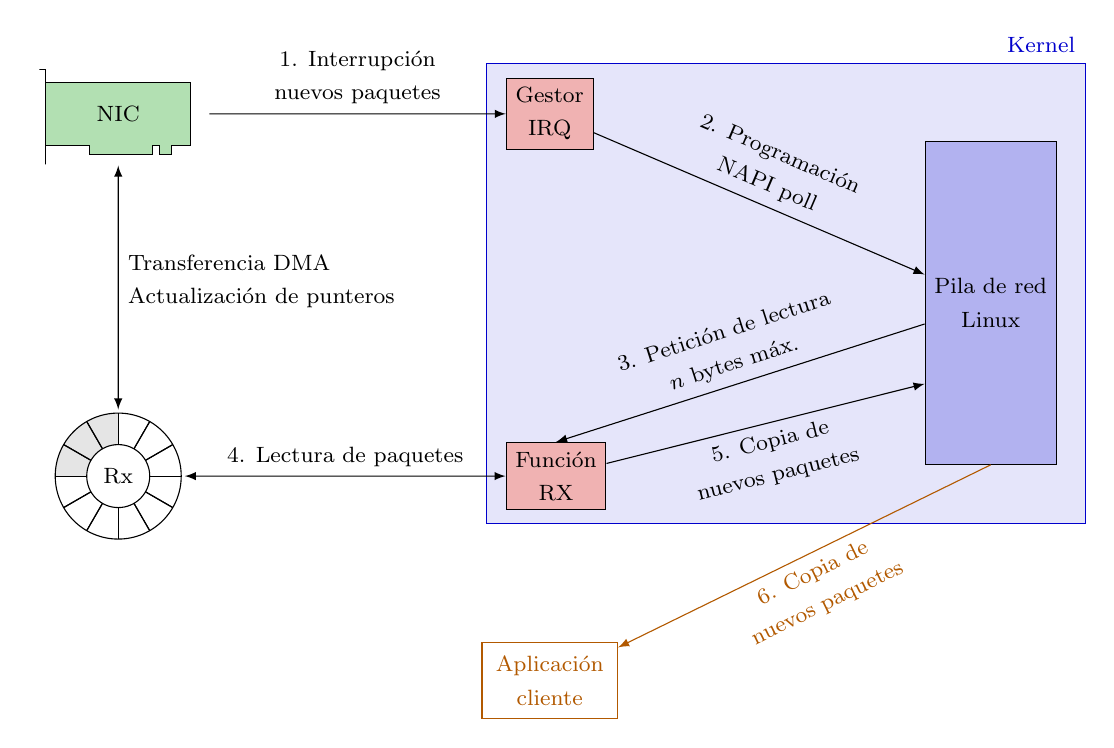
\begin{tikzpicture}[font = {\fontsize{8pt}{12}\selectfont}, scale = 0.8]
\begin{scope}[yshift = 4cm]
\draw[fill = green!60!black, fill opacity = 0.3] (-0.1, 1.2) -- (0, 1.2) -- (0,-0.3) -- (0,0) -- (0.7,0) -- (0.7,-0.15) -- (1.7, -0.15) -- (1.7, 0) -- (1.8, 0) -- (1.8, -0.15) -- (2, -0.15) -- (2,0) -- (2.3, 0) -- (2.3, 1) -- (0,1) -- (0, 1.2) -- cycle ;

\node[rectangle, minimum width = 2.3cm, minimum height = 1cm] (NIC) at (1.15, 0.5) {NIC};
\end{scope}

\draw[blue!80!black, fill = blue!80!black, fill opacity = 0.1] (7, 5.3) rectangle (16.5, -2);
\node[blue!80!black] at (15.8, 5.6) {Kernel};


\node[draw, fill = red!80!black!30!white, align = center] (IRQ) at (8, 4.5) {Gestor \\ IRQ};
\node[draw, fill = blue!80!black!30!white, minimum height = 4.1cm, minimum width = 1.5cm, align = center] (KRN) at (15, 1.5) {Pila de red \\ Linux};
\node[draw, align = center, fill = red!80!black!30!white] (POLL) at (8.1, -1.25) {Funci\'on \\ RX};

\node[draw, orange!70!black, align = center, inner sep = 5pt] (APP) at (8, -4.5) {Aplicaci\'on \\ cliente};

\coordinate (KRN-Mid) at ($(KRN.west)!0.5!(KRN.south west)$);

\begin{scope}[xshift = 1.15cm, yshift = -1.25cm, rotate = 90]
\fill[gray!20!white] (0,0) -- (0,1) arc (90:0:1cm) -- cycle;
\foreach \x in {0, 30, ..., 360}
	\draw ({cos(\x)}, {sin(\x)}) -- ({-cos(\x)}, {-sin(\x)});
\draw (0,0) circle [radius = 1cm];
\draw[black, fill = white] (0,0) circle [radius = 0.5cm]; % Poor man's \clip for intersecting regions
\node[circle, inner sep = 0.45cm] (RNG) at (0,0) {Rx};
\end{scope}

\draw[->] (NIC) --
	node[midway, above, align = center, sloped] {1. Interrupci\'on \\ nuevos paquetes}
	(IRQ);

\draw[->] (IRQ) --
	node[midway, above, sloped, align = center] {2. Programaci\'on \\ NAPI poll}
	(KRN);

\draw[->] (KRN) --
	node[midway, above, sloped, align = center] {3. Petici\'on de lectura \\ $n$ bytes m\'ax.}
	(POLL.north);

\draw[<->, shorten <= 0.15cm] (NIC) --
	node[midway, right, align = left] {Transferencia DMA \\ Actualizaci\'on de punteros}
	(RNG);

\draw[<->] (POLL) -- node[midway, above, align = center, sloped] {4. Lectura de paquetes}
	(RNG);

\draw[->] (POLL) --
	node[midway, below, align = center, sloped] {5. Copia de \\ nuevos paquetes}
	(KRN-Mid);

\draw[<-, orange!70!black] (APP) --
	node[midway, below, sloped, align = center] {6. Copia de  \\ nuevos paquetes}
	(KRN.south);
\end{tikzpicture}

\caption[Funcionamiento de un \textit{driver} de red en Linux]{Esquema del funcionamiento de un \textit{driver} de red en Linux. En rojo, las funciones pertenecientes al \textit{driver}.}
\label{fig:LinuxNetworkStack}
\end{figure}

A grandes rasgos, el funcionamiento de un \textit{driver} de red en Linux es el que aparece en la \fref{fig:LinuxNetworkStack}. Cuando la \gls{nic} recibe nuevos paquetes, emite una \gls{irq} que es recibida por la función correspondiente configurada por el \textit{driver}. Éste se comunica con la pila de red del \textit{kernel} de Linux, más concretamente con el subsistema \gls{NAPI} \cite{NAPI}, avisando de la disponibilidad de nuevos paquetes. Además, desactivará las interrupciones de la tarjeta hasta que no se hayan leído todos los paquetes pendientes, para mejorar así el rendimiento.

El subsistema \gls{NAPI} programará una llamada a la función de recepción del \textit{driver} en función de la carga del sistema, pidiendo la lectura de hasta un cierto máximo de bytes. Cuando esa llamada se realice, el \textit{driver} leerá de una región de memoria los paquetes que la tarjeta haya copiado a través de transferencias DMA, y los transferirá a la pila de red de Linux, que a su vez los gestionará y distribuirá a las aplicaciones cliente correspondientes.

Si bien esta arquitectura es muy efectiva para un sistema de propósito general, tiene varias desventajas como sistema de captura de alto rendimiento. Por un lado, se introduce una cierta latencia al tener que esperar a la primera interrupción y a la llamada correspondiente del subsistema NAPI para empezar a leer los paquetes del anillo de recepción de la tarjeta. Por otra, se realizan dos copias redundantes: del anillo de recepción a la pila de red de Linux y de ésta a la aplicación cliente.

\subsection{HPCAP}

\chapter{Desarrollo e implementación}

\section{Arquitectura Mellanox}

cq (completion queue?), rx rings.

\section{Arquitectura}

\subsection{Hilos}
\label{sec:Hilos}

Varias posibilidades:

\begin{enumerate}
\item Separación del \textit{buffer} de la tarjeta en $n$ partes, cada hilo sólo se preocupa de una de esas partes. La tasa efectiva se reduce a $40 / n$ Gbps por hilo. El problema es que el anillo de la tarjeta se separa en paquetes y el buffer de HPCAP en bytes, así que un segmento de la tarjeta no tiene por qué corresponderse con otro segmento en el buffer.
\item Múltiples hilos escribiendo en el mismo buffer y leyendo del mismo anillo(s). Aquí habría que investigar una forma de sincronización eficiente, usando colas sin bloqueos. Un ejemplo interesante a leer es \href{http://disruptor.googlecode.com/files/Disruptor-1.0.pdf}{Disruptor}. Habría que investigar más bibliografía.
\item Como variación del anterior, múltiples hilos escribiendo en el mismo buffer pero leyendo de segmentos separados del anillo. Así quizás podemos evitar problemas de concurrencia a tasas bajas.
\end{enumerate}

Relacionado con las tasas bajas, una posibilidad con prioridad muy baja es mirar si se puede plantear creación dinámica de hilos según la tasa de recepción, de tal forma que entre el buffer y la creación dinámica se puedan ahorrar recursos en instalaciones con tasa suficientemente baja y sólo con picos de 40Gbps.

\subsection{Filtrado}

Estudiar filtros hardware y posibilidad de filtros software para reducir la tasa de tráfico recibida por la aplicación en espacio de usuario.

\subsection{Almacenamiento y selección de información}

Realizar un estudio teórico de necesidades de almacenamiento según tasa a la que queramos almacenar, viendo productos existentes en el mercado y calculando coste del sistema.

Estudiar si el driver puede realizar un prefiltrado de información en tiempo de recepción, extrayendo sólo ciertos campos de cada paquete. La extracción no debe de ser muy compleja y probablemente tenga que limitarse a extraer ciertos rangos fijos de bytes.

\section{Herramientas adicionales}

\textit{hpcap-test, hpcap-benchmark}.

\chapter{Pruebas}

\section{Caso base: ¿hasta dónde llega la arquitectura básica?}

\begin{figure}[btp]
%\inputgnuplot{gnuplot/simple-arch-max-rate}
\caption[Capacidad de una arquitectura básica de captura]{Una medida de la capacidad base de la tarjeta: tasa máxima que se alcanza sin perder paquetes en función del tamaño de paquetes.}
\label{fig:SimpleArch:MaxRate}
\end{figure}

Dadas las limitaciones del \textit{hardware}, está claro que un único hilo de recepción no será suficiente para hacer la recepción a 40 Gbps. Aun así, es necesario realizar las pruebas en esta arquitectura simple para establecer una base sobre la que comparar y medir mejoras.

Tal y como se ve en la \fref{fig:SimpleArch:MaxRate}, sólo se llega a la tasa máxima de captura a partir de los 1250 bytes de tamaño de paquete. Para tamaños pequeños se observa el mismo comportamiento que con la versión original de HPCAP \citep{MorenoTFM2012}, donde para tamaños cercanos al mínimo (64 bytes) no se llegaba a la tasa máxima de 10 Gbps. En nuestro caso, para ese mismo tamaño se llega a una tasa de 7.6 Gbps.

Así mismo, sobre esta arquitectura básica se ha comprobado el efecto de las marcas de tiempo (\textit{timestamp}) obtenidas a través de la tarjeta o a través del reloj \textit{software} del \textit{kernel} Linux. El rendimiento en ambos casos es prácticamente el mismo.


\chapter{Conclusiones}

\appendix

\printnoidxglossaries
\cleardoublepage

\nocite{*}
\bibliography{hpcap40g}{}

\cleardoublepage
\printindex

\end{document}
